\medskip

Toutes les probabilités, sauf indication contraire, seront arrondies à $10^{-3}$ dans cet exercice.

\og Le virus du chikungunya, transmis à l'homme par la piqûre du moustique tigre provoque chez les patients des douleurs articulaires aiguës qui peuvent être persistantes. En 2005, une importante épidémie de chikungunya a touché les îles de l'Océan Indien et notamment l'île de La Réunion, avec plusieurs centaines de milliers de cas déclarés. En 2007, la maladie a fait son apparition en Europe, puis fin 2013, aux Antilles et a atteint le continent américain en 2014 \fg{}.

\emph{(\href{https://www.pasteur.fr/fr/centre-medical/fiches-maladies/chikungunya}{https://www.pasteur.fr/fr/centre-medical/fiches-maladies/chikungunya})}

Un test a été mis au point pour le dépistage de ce virus.

Le laboratoire fabriquant ce test fournit les caractéristiques suivantes :

\begin{itemize}
\item la probabilité qu'un individu atteint par le virus ait un test positif est de $0,999$ ;
\item la probabilité qu'un individu non atteint par le virus ait un test positif est de $0,005$.
\end{itemize}

On procède à un test de dépistage systématique dans une population cible.

Un individu est choisi au hasard dans cette population. On appelle :

\begin{itemize}
\item $M$ l'évènement : \og l'individu choisi est atteint du chikungunya \fg.
\item $T$ l'évènement : \og le test de l'individu choisi est positif \fg.
\end{itemize}

On considère que le test est \emph{fiable} lorsque la probabilité qu'un individu ayant un test positif soit atteint par le virus est supérieure à $0,95$.

\bigskip

\textbf{Partie A : Étude d'un exemple}

\begin{enumerate}
\item Donner les probabilités $P_{M}(T)$ et $P_{\overline{M}}(T)$.
\end{enumerate} 

\og En mars 2005, l'épidémie s'est propagée rapidement dans l'ile de La Réunion, avec une flambée importante entre fin avril et début juin puis une persistance de la transmission virale durant l'hiver austral. Au total, $\np{270000}$ personnes ont été infectées pour une population totale de $\np{750000}$ individus \fg{}.\\
\emph{(\href{https://www.pasteur.fr/fr/centre-medical/fiches-maladies/chikungunya}{https://www.pasteur.fr/fr/centre-medical/fiches-maladies/chikungunya})}

Fin 2005, le laboratoire a effectué un test de dépistage massif de la population de l'île de La Réunion.\\
 Dans cette partie, la population cible est donc la population de l'ile de La Réunion.


\begin{enumerate}[resume]
\item Donner la valeur exacte de $P(M)$.
\item  Recopier et compléter l'arbre pondéré donné ci-dessous. 

\hfill~
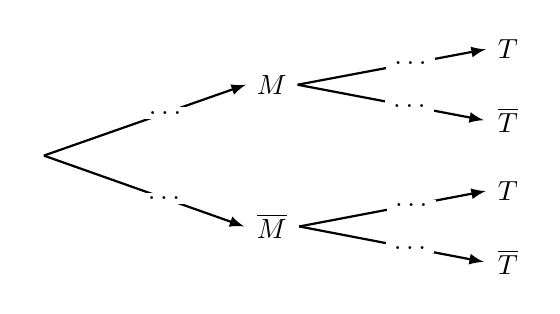
\begin{tikzpicture}[xscale=1,yscale=1,baseline={(R.base)}]
	\tikzstyle{fleche}=[->,>=latex,thick]
	\tikzstyle{noeud}=[fill=white,circle,inner sep=2pt]
	\tikzstyle{feuille}=[fill=white,circle,inner sep=2pt]
	\tikzstyle{etiquette}=[pos=0.6,fill=white, inner xsep=3pt, inner ysep=1.5pt]
	\def\DistanceInterNiveaux{3}
	\def\DistanceInterFeuilles{0.9}
	\def\NiveauA{(0)*\DistanceInterNiveaux}
	\def\NiveauB{(1)*\DistanceInterNiveaux}
	\def\NiveauC{(2)*\DistanceInterNiveaux}
	\def\InterFeuilles{(-1)*\DistanceInterFeuilles}
	
	\node[noeud] (R) at ({\NiveauA},{(1.5)*\InterFeuilles}) {};
	\node[noeud] (Ra) at ({\NiveauB},{(0.5)*\InterFeuilles}) {$M$};
	\node[feuille] (Raa) at ({\NiveauC},{(0)*\InterFeuilles}) {$T$};
	\node[feuille] (Rab) at ({\NiveauC},{(1)*\InterFeuilles}) {$\overline{T}$};
	\node[noeud] (Rb) at ({\NiveauB},{(2.5)*\InterFeuilles}) {$\overline{M}$};
	\node[feuille] (Rba) at ({\NiveauC},{(2)*\InterFeuilles}) {$T$};
	\node[feuille] (Rbb) at ({\NiveauC},{(3)*\InterFeuilles}) {$\overline{T}$};
	
	\draw[fleche] (R.east)--(Ra.west) node[etiquette] {$\ldots$};
	\draw[fleche] (Ra.east)--(Raa.west) node[etiquette] {$\ldots$};
	\draw[fleche] (Ra.east)--(Rab.west) node[etiquette] {$\ldots$};
	\draw[fleche] (R.east)--(Rb.west) node[etiquette] {$\ldots$};
	\draw[fleche] (Rb.east)--(Rba.west) node[etiquette] {$\ldots$};
	\draw[fleche] (Rb.east)--(Rbb.west) node[etiquette] {$\ldots$};
\end{tikzpicture} \hfill~

\item Calculer la probabilité qu'un individu soit atteint par le virus et ait un test positif.
\item  Calculer la probabilité qu'un individu ait un test positif.
\item  Calculer la probabilité qu'un individu ayant un test positif soit atteint par le virus.
\item  Peut-on estimer que ce test est fiable? Argumenter.
\end{enumerate}

\textbf{Partie B : Dépistage sur une population cible}

\medskip

Dans cette partie, on note $p$ la proportion de personnes atteintes par le virus du chikungunya dans une population cible.\\
On cherche ici à tester la fiabilité du test de ce laboratoire en fonction de $p$.

\begin{enumerate}
\item Recopier, en l'adaptant, l'arbre pondéré de la question A3 en tenant compte des nouvelles données.
\item Exprimer la probabilité $P(T)$ en fonction de $p$.
\item Montrer que $P_{T}(M) = \dfrac{999 p}{994 p+5}$.
\item Pour quelles valeurs de $p$ peut-on considérer que ce test est fiable?
\end{enumerate}

\textbf{Partie C : Étude sur un échantillon}

\medskip

Pendant l'épidémie, on admet que la probabilité d'être atteint du chikungunya sur l'ile de La Réunion est de 0,36.

On considère un échantillon de $n$ individus choisis au hasard, en assimilant ce choix à un tirage au sort avec remise. On désigne par $X$ la variable aléatoire dénombrant le nombre d'individus infectés dans cet échantillon parmi les $n$ tirés au sort.

On admet que $X$ suit une loi binomiale de paramètres $n$ et $p=0,36$.


Déterminer à partir de combien d'individus $n$ la probabilité de l'évènement \og au moins un des $n$ habitants de cet échantillon est atteint par le virus \fg est supérieure à $0,99$. Expliquer la démarche.

\bigskip
